\Variant{23.02.2025 (1-smena)}
\QQ{1}{$a$, $b$, $c$, $d$, $f$ turli raqamlar bölib, $\overline{aaaa}-\overline{bbb}+\overline{cc}+d+f=5000$ bölsa, $a\cdot b-d\cdot f+c$ ning qiymatini toping.
\Opts{$4$}{$9$}{$7$}{$5$}}
\QQ{2}{Hisoblang:
\[\left(4{,}(6)\cdot2\frac47-3\right)\cdot1{,}0(5)-\frac1{0{,}4}\]
\Opts{$6$}{$7$}{$9{,}5$}{$7{,}5$}}
\QQ{3}{Basseynda $4$ ta quvur bor. Birinçi va ikkinçi quvur basseynni töldiradi. Uçinçi va törtinçi quvur basseynni böşatadi. $4$ ta quvur birdaniga oçilsa basseyn $5$ soatda töladi. Faqat birinçi, ikkinçi va uçinçi quvurlar oçilsa $3$ soatda töladi. Faqat birinçi, uçinçi va törtinçi quvurlar oçilsa $30$ soatda töladi. Faqat birinçi va uçinçi quvurlar oçilsa basseyn neça soatda töladi?
\Opts{$10$ soat}{$4$ soat}{$6$ soat}{$5$ soat}}
\QQ{4}{Köylakning narxi $100\,000$ söm edi. Dastlab köylak narxi $10\%$ ga oşirildi, keyin $15\%$ ga arzonlaştirildi. Köylakning hozirgi narxini toping.
\Opts{$93\,500$}{$103\,500$}{$92\,000$}{$95\,000$}}
\QQ{5}{Agar $x>0$, $x^2=2048^{24}$ va $\sqrt[3]y=512^5$ bölsa, $\dfrac xy$ ni toping.
\Opts{$8$}{$\dfrac18$}{$64$}{$\dfrac1{64}$}}
\QQ{6}{Soddalaştiring:
\[\frac{\left(\sqrt{11}-\sqrt5\right)\left(\sqrt{15}+\sqrt{33}-\sqrt{22}-\sqrt{10}\right)}{\sqrt{108}-\sqrt{72}}\]
\Opts{$1$}{$2$}{$3$}{$4$}}
\QQ{7}{Kasr maxrajini irratsionallikdan qutqaring:
\[\frac1{\sqrt2+\sqrt3-\sqrt5}\]
\Opts{$\dfrac{3\sqrt2+2\sqrt3+\sqrt{30}}6$}{$\dfrac{3\sqrt2+2\sqrt3+\sqrt{30}}{12}$}{$\dfrac{3\sqrt2+2\sqrt3-\sqrt{30}}{12}$}{$\dfrac{3\sqrt2-2\sqrt3+\sqrt{30}}{12}$}}
\QQ{8}{Arifmetik progressiyada $a_{14}=20$ va $S_{28}=600$ ga teng bölsa, $a_{28}$ ni toping.
\Opts{$60$}{$40$}{$70$}{$80$}}
\QQ{9}{Kamayuvçi geometrik progressiyada dastlabki $3$ ta hadi yiğindisi $14$ ga, ularning kvadratlari yiğindisi $84$ ga teng bölsa, progressiyaning dastlabki $6$ ta hadi yiğindisini toping.
\Opts{$15\dfrac34$}{$14\dfrac34$}{$13\dfrac23$}{$12\dfrac15$}}
\QQ{10}{$P(0;\,1)$ nuqtani $3$ radianga buriş natijasida hosil bölgan nuqta qaysi çorakda yotadi?
\Opts{II}{III}{I}{IV}}
\QQ{11}{Agar $|c|<|b|<|a|$ va $a<0$, $b>0$, $c<0$ bölsa, $\dfrac{a|b-c|}{|a|}+\dfrac{b|c-a|}{|b|}+\dfrac{c|a-b|}{|c|}$ ni hisoblang.
\Opts{$2a-2b$}{$0$}{$2c-2a$}{$2c-2b$}}
\QQ{12}{Ifodani soddalaştiring:
\[\frac{-4\cdot4^{x-1}\cdot3^{2x+1}-12^{x+1}\cdot3^{x+2}}{36^x\cdot8+9^x\cdot2^{2x+1}}\]
\Opts{$11{,}1$}{$10{,}1$}{$-11{,}1$}{$-10{,}1$}}
\QQ{13}{Ifodani soddalaştiring:
\[\frac{\sin^22\alpha\cdot\tg^22\alpha}{1-\ctg^22\alpha}+\frac{\cos^22\alpha\cdot\ctg^22\alpha}{1-\tg^22\alpha}+2\]
\Opts{$\tg^22\alpha-\ctg^22\alpha$}{$\dfrac2{\tg^22\alpha-\ctg^22\alpha}$}{$\dfrac4{\sin^24\alpha}$}{$\tg^22\alpha+\ctg^22\alpha+1$}}
\QQ{14}{Tengsizlikni yeçing:
\[3^x-2^{x+2}+2^{x-3}+2^{x-1}-3^{x-1}\ge0\]
\Opts{$(5;\,\infty)$}{$(4;\,\infty)$}{$[4;\,\infty)$}{$[5;\,\infty)$}}
\QQ{15}{Ifodaning qiymatini toping:
\[2023^{\log^2_{2023}2024}-2024^{\log_{2023}2024}-\log_2\log_2\underbrace{\sqrt{\sqrt{\sqrt{\dots\sqrt2}}}}_{2023\ \text{ta}}\]
\Opts{$2024$}{$-2023$}{$-2024$}{$2023$}}
\QQ{16}{Tenglama neçta haqiqiy ildizga ega?
\[\frac{(x+2)^2-9}{x+7}\cdot(x+7)=16\]
\Opts{$1$}{$2$}{$3$}{yeçimga ega emas}}
\QQ{17}{Tenglamaning haqiqiy ildizlari köpaytmasini toping:
\[(x-3)^2+3x=\sqrt{x^2-3x+7}+22\]
\Opts{$162$}{$-18$}{$-9$}{$-162$}}
\QQ{18}{$2x^2+2\sqrt2x+1\le0$ tengsizlik neçta yeçimga ega?
\Opts{$1$}{$2$}{$0$}{çeksiz köp}}
\QQ{19}{Tengsizlikni qanoatlantiruvçi butun sonlar yiğindisini toping:
\[\frac{x^2-5x+64}{x^2-10x+24}\le\frac{10}{4-x}\]
\Opts{$0$}{$10$}{$5$}{$-5$}}
\QQ{20}{Neçta natural son $f(x)=6\sin x-4\cos x$ funksiyaning qiymatlar sohasiga tegişli?
\Opts{$15$}{$7$}{$4$}{$14$}}
\QQ{21}{$y=x^2-\left(a^2-2a-3\right)x+6$ funksiya nollari $x=2$ va $x=3$ ga teng böladigan $a$ ning qiymatlarini toping.
\Opts{$1;\ 2$}{$-2;\ 1$}{$4;\ -2$}{$0;\ 2$}}
\QQ{22}{Agar $f(x)=\left|\log_{\cos x}\sin x-\ln\pi\right|$ bölsa, $f'\left(\dfrac\pi4\right)$ ni toping.
\Opts{$\log_2e$}{$-4\log_2e$}{$-4\log_4e$}{$4\log_2e$}}
\QQ{23}{Aniq integralni hisoblang:
\[\int_2^4\frac3{5-4x-x^2}\,dx\]
\Opts{$\ln\dfrac37$}{$\ln\sqrt{\dfrac37}$}{$\ln\sqrt{\dfrac73}$}{$\ln\dfrac73$}}
\QQ{24}{$ABC$ uçburçakka içki çizilgan aylana uçburçakning $AB$, $BC$ va $AC$ tomonlariga mos ravişda $F$, $D$ va $E$ nuqtalarda urinadi. Agar $|AB|=9$, $|BC|=7$ va $|AC|=10$ ga teng bölsa, $AE$ kesma uzunligini toping.
\qfig{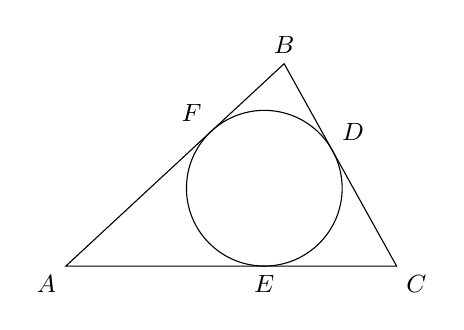
\begin{tikzpicture}[scale=0.42,font=\small]
\coordinate (A) at (0,0); \coordinate (C) at (10,0); \coordinate (B) at (6.6,6.119); \coordinate (I) at (6,2.354);
\coordinate (F) at (4.4,4.079); \coordinate (D) at (8.057,3.497); \coordinate (E) at (6,0);
\draw (A)--(B)--(C)--cycle; \draw (I) circle (2.354);
\node[below left] at (A) {$A$}; \node[above] at (B) {$B$}; \node[below right] at (C) {$C$};
\node[above left] at (F) {$F$}; \node[above right] at (D) {$D$}; \node[below] at (E) {$E$};
\end{tikzpicture}}
\Opts{$4$}{$6$}{$8$}{$5$}}
\QQ{25}{$ABC$ töğri burçakli uçburçak gipotenuzasi uzunligi $15$ ga, $\sin\angle ACB=0{,}6$ ga teng bölsa, uçburçak yuzini toping.
\qfig{\begin{tikzpicture}[scale=0.3,font=\small]
\coordinate (A) at (0,0); \coordinate (C) at (12,0); \coordinate (B) at (0,9);
\draw (A)--(B)--(C)--cycle; \draw (0,0.7)--(0.7,0.7)--(0.7,0);
\draw (C)+(143.13:1.5) arc (143.13:180:1.5);
\node[below left] at (A) {$A$}; \node[above left] at (B) {$B$}; \node[below right] at (C) {$C$};
\node[above right] at (6,4.5) {$15$}; \node at (9.6,0.5) {\scriptsize$\alpha$};
\end{tikzpicture}}
\Opts{$56$}{$54$}{$108$}{$36$}}
\QQ{26}{$ABC$ töğri burçakli uçburçakka $ADEF$ kvadrat şunday içki çizilganki, ular uçun töğri burçak umumiy va $A$ burçagi töğri. Agar $|BE|=20$, $|EC|=30$ ga teng bölsa, böyalgan soha yuzini toping.
\qfig{\begin{tikzpicture}[scale=0.1,font=\small]
\coordinate (A) at (0,0); \coordinate (D) at (0,16.64); \coordinate (B) at (0,27.73); \coordinate (E) at (16.64,16.64); \coordinate (F) at (16.64,0); \coordinate (C) at (41.6,0);
\fill[qfill] (B)--(D)--(E)--cycle; \fill[qfill] (E)--(F)--(C)--cycle;
\draw (A)--(B)--(C)--cycle; \draw (D)--(E)--(F); \draw (0,2)--(2,2)--(2,0);
\node[below left] at (A) {$A$}; \node[above left] at (B) {$B$}; \node[left] at (D) {$D$}; \node[above right] at (E) {$E$}; \node[below] at (F) {$F$}; \node[below right] at (C) {$C$};
\node[above right] at (8.3,22.2) {$20$}; \node[above right] at (29,8.3) {$30$};
\end{tikzpicture}}
\Opts{$600$}{$325$}{$300$}{$225$}}
\QQ{27}{$ABCD$ kvadrat tomoni uzunligi $6$ ga teng. $AF=2$, $CE=3$, $\angle FMA=b$, $\angle CNE=a$ bölsa, $a+b$ ni toping.
\qfig{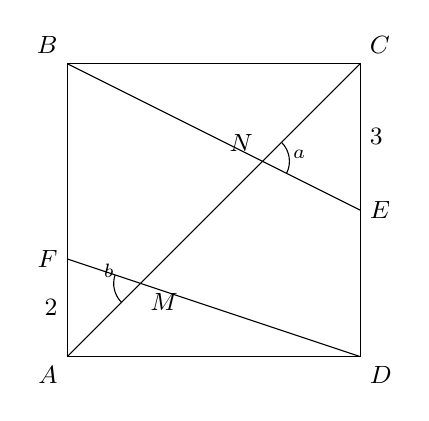
\begin{tikzpicture}[scale=0.62,font=\small]
\coordinate (A) at (0,0); \coordinate (B) at (0,6); \coordinate (C) at (6,6); \coordinate (D) at (6,0); \coordinate (F) at (0,2); \coordinate (E) at (6,3); \coordinate (M) at (1.5,1.5); \coordinate (N) at (4,4);
\draw (A)--(B)--(C)--(D)--cycle; \draw (A)--(C); \draw (F)--(D); \draw (B)--(E);
\draw (M)+(161.57:0.55) arc (161.57:225:0.55); \draw (N)+(-26.57:0.55) arc (-26.57:45:0.55);
\node[below left] at (A) {$A$}; \node[above left] at (B) {$B$}; \node[above right] at (C) {$C$}; \node[below right] at (D) {$D$}; \node[left] at (F) {$F$}; \node[right] at (E) {$E$};
\node[below right] at (M) {$M$}; \node[above left] at (N) {$N$}; \node at (0.85,1.75) {\scriptsize$b$}; \node at (4.75,4.15) {\scriptsize$a$};
\node[left] at (0,1) {$2$}; \node[right] at (6,4.5) {$3$};
\end{tikzpicture}}
\Opts{$115^\circ$}{$135^\circ$}{$150^\circ$}{$120^\circ$}}
\QQ{28}{Taşqi burçagi $45^\circ$ ga teng bölgan muntazam köpburçakka aylana taşqi çizilgan. Aylana radiusi $2$ ga teng bölsa, köpburçak yuzini toping.
\Opts{$4\sqrt2$}{$\sqrt2$}{$6\sqrt2$}{$8\sqrt2$}}
\QQ{29}{Özaro $120^\circ$ li burçak taşkil qiluvçi ikki yoqli tekislik berilgan. $A$ va $C$ nuqtalar qirrada, $B$ va $D$ nuqtalar mos ravişda yoqlarda yotadi. Agar $|AC|=7\sqrt3$, $|AB|=12$, $|DC|=4\sqrt3$, $\angle BAC=30^\circ$ va $\angle ACD=60^\circ$ bölsa, $B$ va $D$ nuqtalar orasidagi masofani toping.
\qfig{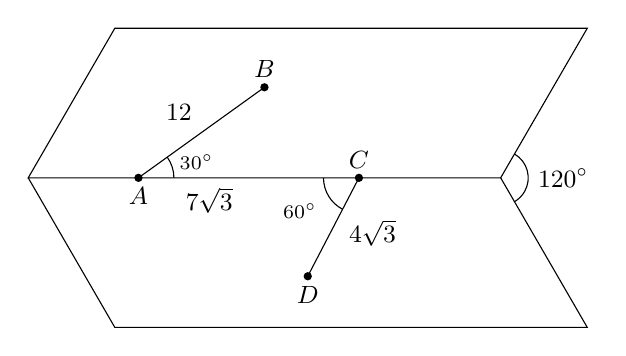
\begin{tikzpicture}[scale=1.0,font=\small]
\draw (0,0)--(1.1,1.9)--(7.1,1.9)--(6,0)--cycle; \draw (0,0)--(1.1,-1.9)--(7.1,-1.9)--(6,0);
\coordinate (A) at (1.4,0); \coordinate (B) at (3.0,1.15); \coordinate (C) at (4.2,0); \coordinate (D) at (3.55,-1.25);
\draw (A)--(B); \draw (C)--(D); \fill (A) circle (1.5pt); \fill (B) circle (1.5pt); \fill (C) circle (1.5pt); \fill (D) circle (1.5pt);
\draw (A)+(0:0.45) arc (0:35.7:0.45); \draw (C)+(180:0.45) arc (180:242.5:0.45); \draw (6,0)+(60:0.35) arc (60:-60:0.35);
\node[below] at (A) {$A$}; \node[above] at (B) {$B$}; \node[above] at (C) {$C$}; \node[below] at (D) {$D$};
\node[above left] at (2.2,0.6) {$12$}; \node[below] at (2.3,0) {$7\sqrt3$}; \node[right] at (3.95,-0.7) {$4\sqrt3$};
\node[right] at (1.8,0.2) {\scriptsize$30^\circ$}; \node at (3.45,-0.42) {\scriptsize$60^\circ$}; \node[right] at (6.35,0) {$120^\circ$};
\end{tikzpicture}}
\Opts{$6\sqrt3$}{$12$}{$\sqrt{75+6\sqrt{39}}$}{$\sqrt{111}$}}
\QQ{30}{Rasmda $x^2+y^2=36$ aylana va $y=kx+b$ töğri çiziq grafiklari tasvirlangan. $B$ nuqtadan $OX$ öqigaça bölgan eng qisqa masofani toping.
\qfig{\begin{tikzpicture}[scale=0.3,font=\small]
\draw[-{Stealth[length=4pt]}] (-9,0)--(9,0) node[right] {$x$}; \draw[-{Stealth[length=4pt]}] (0,-8)--(0,8.5) node[left] {$y$};
\draw (0,0) circle (6); \draw (-7.2,-0.69)--(7.5,7.79) node[right] {$y=kx+b$};
\fill (-6,0) circle (5pt); \fill (3,5.196) circle (5pt);
\draw (-6,0)+(0:1.6) arc (0:30:1.6);
\node[below left] at (-6,0) {$A$}; \node[above] at (3,5.4) {$B$}; \node[below left] at (0,0) {$O$}; \node[right] at (-4.3,0.5) {\scriptsize$30^\circ$};
\end{tikzpicture}}
\Opts{$6$}{$3\sqrt3$}{$3$}{$6\sqrt3$}}
\QQ{31}{Quyidagi universal töplam içida $A$ va $B$ töplamlar berilgan. $(A\cup B)'\cup A$ töplamning qism töplamlari sonini toping.
\qfig{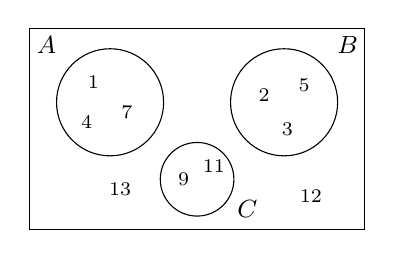
\begin{tikzpicture}[scale=0.85,font=\small]
\draw (0,0) rectangle (5,3);
\draw (1.2,1.9) circle (0.8); \draw (3.8,1.9) circle (0.8); \draw (2.5,0.75) circle (0.55);
\node at (0.25,2.75) {$A$}; \node at (4.75,2.75) {$B$}; \node at (3.25,0.3) {$C$};
\node at (0.95,2.2) {\scriptsize1}; \node at (0.85,1.6) {\scriptsize4}; \node at (1.45,1.75) {\scriptsize7};
\node at (3.5,2.0) {\scriptsize2}; \node at (4.1,2.15) {\scriptsize5}; \node at (3.85,1.5) {\scriptsize3};
\node at (2.3,0.75) {\scriptsize9}; \node at (2.75,0.95) {\scriptsize11}; \node at (1.35,0.6) {\scriptsize13}; \node at (4.2,0.5) {\scriptsize12};
\end{tikzpicture}}
\Opts{$128$}{$64$}{$256$}{$32$}}
\QQ{32}{Barça raqamlari toq bölgan, uçga karrali uç xonali sonlar neçta?
\Opts{$35$}{$36$}{$41$}{$29$}}
\QQ{33}{\Moslash{Çodirning tomi konusdan, pastki qismi silindrdan iborat. Konus va silindr asoslari ustma-ust tuşadi va balandliklari bir xil. Çodirning balandligi $6$ ga teng bölsa,
\par\centering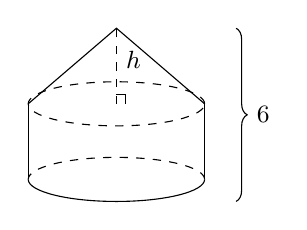
\begin{tikzpicture}[scale=0.8,font=\small]
\draw (-1.4,0)--(-1.4,1.2); \draw (1.4,0)--(1.4,1.2); \draw (-1.4,0) arc (180:360:1.4 and 0.35); \draw[dashed] (1.4,0) arc (0:180:1.4 and 0.35);
\draw[dashed] (0,1.2) ellipse (1.4 and 0.35); \draw (-1.4,1.2)--(0,2.4)--(1.4,1.2); \draw[dashed] (0,1.2)--(0,2.4); \draw (0,1.35)--(0.15,1.35)--(0.15,1.2);
\node[right] at (0,1.9) {$h$}; \draw [decorate,decoration={brace,amplitude=4pt}] (1.9,2.4)--(1.9,-0.35) node[midway,right=4pt] {$6$};
\end{tikzpicture}}{A) $64\pi$\par B) $68\pi$\par C) $54\pi$\par D) $56\pi$\par E) $60\pi$\par F) $72\pi$}{Çodirning tom qismini qoplaş uçun $20\pi$ (m$^2$) gazlama ketgan bölsa, çodirning hajmini toping.}{Konusning hajmi $81\pi$ (m$^3$) bölsa, silindr yon sirtini toping.}{Konus yasovçisi konus asosi radiusidan $\dfrac{\sqrt{17}}4$ marta katta bölsa, silindr yon sirtini toping.}}
\QQ{36}{$x^4-4x^3-4x^2+16x-8=0$ tenglama berilgan.
\AB{Tenglamaning haqiqiy ildizlari neçta?}{Tenglamaning haqiqiy ildizlari $x_1$, $x_2$, \dots, $x_n$ bölsa, $|x_1|+|x_2|+\dots+|x_n|$ ni toping.}}
\QQ{37}{Agar
\[\begin{cases}\tg x+\tg\dfrac y2=\dfrac4{\sqrt3}\\[2mm] \ctg x+\ctg\dfrac y2=\dfrac4{\sqrt3}\end{cases}\]
bölsa,
\AB{$\tg y$ ning eng kiçik qiymatini toping.}{$x$ ning eng kiçik musbat qiymatini toping.}}
\QQ{38}{$f(x)+\dfrac{x-1}{2x+1}\cdot f\left(\dfrac1x\right)=\dfrac3{x-1}$ funksiya berilgan bölsa,
\AB{$f(2)$ ning qiymatini toping.}{$f(x)=0$ tenglamaning ildizlari yiğindisini (agar tenglama ildizi bitta bölsa, şu ildizini) toping.}}
\QQ{39}{Rasmda $y=f(x)$ grafigi tasvirlangan.
\qfig{\begin{tikzpicture}[x=0.45cm,y=0.65cm,font=\small]
\draw[-{Stealth[length=4pt]}] (-7,0)--(7.2,0) node[right] {$x$}; \draw[-{Stealth[length=4pt]}] (0,-2.4)--(0,3.4) node[right] {$y$};
\draw[thick] plot[smooth,tension=0.6] coordinates {(-6,1.3) (-5.2,2.1) (-4,0) (-2.4,-1.6) (-1.3,-0.6) (-0.1,2.7) (0.9,0.6) (1.85,-0.5) (3.3,2) (4.9,-1.85) (6,0.6)};
\draw[dashed] (-6,0)--(-6,1.3);
\node[below] at (-6,0) {$-6$}; \node[below] at (6.2,0) {$6$}; \node[right] at (1.2,2.9) {$y=f(x)$};
\end{tikzpicture}}
\AB{$f(x)$ funksiyaning $(-6;\,6)$ oraliqda neçta lokal maksimum nuqtasi bor?}{$f'(x)=0$ tenglamaning $(-6;\,6)$ oraliqdagi ildizlari sonini toping.}}
\QQ{40}{$y_1=\dfrac{(x+2)^3}{16}$ funksiyaga $x_0=2$ nuqtada urinma ötkazilgan. Bu töğri çiziq $y_2=kx+b$ bölsa,
\qfig{\begin{tikzpicture}[x=0.8cm,y=0.42cm,font=\small]
\fill[qfill] (0,0)--(0,0.5)-- plot[domain=0:2,samples=30] (\x,{(\x+2)^3/16}) --(0.667,0)--cycle;
\draw[-{Stealth[length=4pt]}] (-2.7,0)--(3.6,0) node[right] {$x$}; \draw[-{Stealth[length=4pt]}] (0,-3.3)--(0,7.6) node[left] {$y$};
\draw[thick,domain=-2.6:2.55,samples=60] plot (\x,{(\x+2)^3/16}); \draw (-0.3,-2.9)--(2.75,6.25) node[right] {$y_2=kx+b$};
\draw[dashed] (2,0)--(2,4); \node[below] at (2,0) {$2$};
\node[left] at (-1.6,-2.2) {$y_1=\dfrac{(x+2)^3}{16}$};
\end{tikzpicture}}
\AB{$k\cdot b^2$ ni toping.}{Ştrixlangan soha yuzini toping.}}
\QQ{41}{$ABC$ töğri burçakli uçburçakda $BH$ balandligi uni ikkita $ABH$ va $BCH$ töğri burçakli uçburçaklarga ajratadi. $ABH$ va $BCH$ uçburçaklarga içki çizilgan aylana radiuslari mos ravişda $3$ va $4$ ga teng bölsa,
\qfig{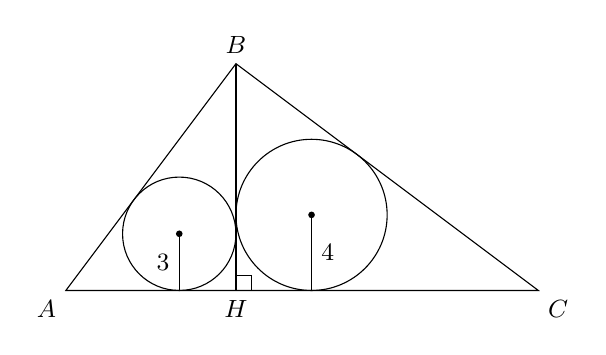
\begin{tikzpicture}[scale=0.24,font=\small]
\coordinate (A) at (0,0); \coordinate (C) at (25,0); \coordinate (H) at (9,0); \coordinate (B) at (9,12);
\draw (A)--(B)--(C)--cycle; \draw (B)--(H); \draw (6,3) circle (3); \draw (13,4) circle (4);
\draw (6,0)--(6,3); \draw (13,0)--(13,4); \fill (6,3) circle (5pt); \fill (13,4) circle (5pt);
\draw (9,0.8)--(9.8,0.8)--(9.8,0);
\node[below left] at (A) {$A$}; \node[above] at (B) {$B$}; \node[below right] at (C) {$C$}; \node[below] at (H) {$H$};
\node[left] at (6,1.5) {$3$}; \node[right] at (13,2) {$4$};
\end{tikzpicture}}
\AB{$BH$ balandlikni toping.}{$ABC$ uçburçakning yuzini toping.}}
\QQ{42}{Tomonlari $6$, $6$, $8$, $8$ ga teng bölgan qavariq törtburçak berilgan va unga içki va taşqi aylanalar çizilgan bölsa,
\qfig{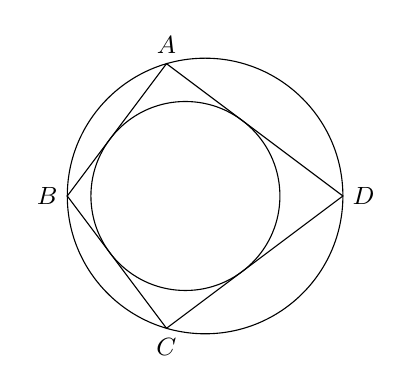
\begin{tikzpicture}[scale=0.35,font=\small]
\coordinate (B) at (-5,0); \coordinate (D) at (5,0); \coordinate (A) at (-1.4,4.8); \coordinate (C) at (-1.4,-4.8);
\draw (0,0) circle (5); \draw (-0.714,0) circle (3.429); \draw (A)--(B)--(C)--(D)--cycle;
\node[above] at (A) {$A$}; \node[left] at (B) {$B$}; \node[below] at (C) {$C$}; \node[right] at (D) {$D$};
\end{tikzpicture}}
\AB{Törtburçakning kiçik diagonalini toping.}{Içki va taşqi çizilgan aylanalar markazlari orasidagi masofani toping.}}
\QQ{43}{$ABCDEF$ qavariq oltiburçakning barça tomonlari $2$ ga teng. $\angle A=\angle E=90^\circ$ va $\angle C=60^\circ$ bölsa,
\qfig{\begin{tikzpicture}[scale=0.85,font=\small]
\coordinate (A) at (-1.823,1.823); \coordinate (B) at (-1,0); \coordinate (C) at (0,-1.732); \coordinate (D) at (1,0); \coordinate (E) at (1.823,1.823); \coordinate (F) at (0,2.646);
\draw (A)--(B)--(C)--(D)--(E)--(F)--cycle;
\node[left] at (A) {$A$}; \node[left] at (B) {$B$}; \node[below] at (C) {$C$}; \node[right] at (D) {$D$}; \node[right] at (E) {$E$}; \node[above] at (F) {$F$};
\end{tikzpicture}}
\AB{$BFD$ uçburçak yuzini toping.}{Oltiburçak tomoni $\dfrac{10}{\sqrt{4+\sqrt7+\sqrt3}}$ bölsa, oltiburçak yuzini toping.}}
\QQ{44}{Şarga konus içki çizilgan. Konus yon sirti $18\sqrt{2+\sqrt3}\,\pi$ ga teng. Konus yasovçisi va asos tekisligi orasidagi burçak $75^\circ$ ga teng bölsa,
\qfig{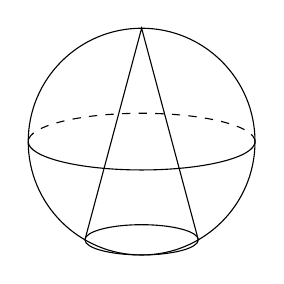
\begin{tikzpicture}[scale=0.24,font=\small]
\draw (0,0) circle (6); \draw (-3,-5.196)--(0,6)--(3,-5.196); \draw (0,-5.196) ellipse (3 and 0.8);
\draw (-6,0) arc (180:360:6 and 1.5); \draw[dashed] (6,0) arc (0:180:6 and 1.5);
\end{tikzpicture}}
\AB{Konus asosining radiusini toping.}{Şar hajmini toping ($\pi\approx3$ deb olinsin).}}
\QQ{45}{Uy hayvonlari uçun yarim silindr şaklidagi temir listdan böyi $200$ cm, diametri $40$ cm suv idişi yasalgan bölsa ($\pi\approx3$ deb olinsin),
\qfig{\begin{tikzpicture}[scale=0.9,font=\small]
\fill[qfill] (0,0)--(2,3)--(3.2,3)--(1.2,0)--cycle; \fill[qfill] (0,0) arc (180:360:0.6) -- cycle; \fill[qfill] (2,3) arc (180:360:0.6)--cycle;
\draw (0,0)--(2,3)--(3.2,3)--(1.2,0)--cycle; \draw (0,0) arc (180:360:0.6); \draw (2,3) arc (180:360:0.6); \draw (1.2,-0.6)--(3.2,2.4);
\draw[dashed] (0.6,0)--(2.6,3);
\draw[{Stealth[length=4pt]}-{Stealth[length=4pt]}] (-0.25,0.15)--(1.75,3.15); \node[rotate=56.3,above] at (0.75,1.65) {\scriptsize$200$ cm};
\draw[{Stealth[length=4pt]}-{Stealth[length=4pt]}] (2,3.25)--(3.2,3.25); \node[above] at (2.6,3.25) {\scriptsize$40$ cm};
\end{tikzpicture}}
\AB{Suv idişini çiqindi çiqmaydigan qilib tayyorlaş uçun qança (dm$^2$) temir list işlatadi?}{Suv idişiga qança litr suv ketadi?}}
\Javoblar{C B C A B A B A A B D C C C D A B A D B C D B B B C B D D B A C A C F}{%
\OK{36}{$4$}{$2+2\sqrt2+2\sqrt3$}\OK{37}{$-\sqrt3$}{$\dfrac\pi6$}\OK{38}{$4$}{$-2$}\OK{39}{$3$}{$6$}\OK{40}{$12$}{$\dfrac{13}{12}$}%
\OK{41}{$12$}{$150$}\OK{42}{$9{,}6$}{$\dfrac57$}\OK{43}{$\sqrt7$}{$25$}\OK{44}{$3$}{$864$}\OK{45}{$132$}{$120$}}
